\documentclass{ximera}

\title{Omzetten van eenheden}
\author{Daan Lipkens}

\begin{document}
\begin{abstract}
    Oppervlakte, volume, samengestelde eenheden (breuken) en tijd omzetten.
\end{abstract}
\maketitle

\section{Het omzetten van oppervlaktematen en volumematen}
Het omzetten van oppervlaktematen en volumematen gebeurt op een analoge manier zoals we in de vorige sectie besproken hebben. Het enige verschil nu is dat je met de rekenregels van machten rekening moet houden.

\begin{example}[title={Invullen van Prefix}]\nl
    Je meet een waarde van $8{,}3 \, \mathrm{cm}^{2}$. Hoeveel meter is dit? Om dit te weten te komen, gaan we op een analoge manier te werk zoals we in de vorige sectie gedaan hebben. We kunnen in de tabel dus aflezen dat centi (c) gelijk is aan $10^{-2}$. De eenheid $\mathrm{cm}^{2}$ lees je als ``vierkante centimeter'', wat hetzelfde is als ``cm tot de tweede''. Met dit in het achterhoofd vinden we bijgevolg dat:
    \begin{align*}
    8{,}3 \, \mathrm{cm}^{2} & = 8{,}3 \, (\mathrm{cm})^{2} \\
    & = 8{,}3 \cdot (10^{-2} \, \mathrm{m})^{2} \\
    & = 8{,}3 \cdot 10^{-4} \, \mathrm{m}^{2}.
    \end{align*}
\end{example}

\begin{example}[foldable=true,title={Voorbeeld: Kubieke meter omzetten naar kubieke micrometer}]\nl
    Je meet een waarde van $3{,}4 \, \mathrm{m}^{3}$. Hoeveel kubieke micrometer is dit?

    \begin{solution}\nl
    In de tabel lees je af dat micro ($\mu$) gelijk is aan $10^{-6}$. Bijgevolg vinden we dat:
    \begin{align*}
    1 \, \mathrm{\mu m}^{3} & = 1 \, (\textcolor{red}{\mathrm{\mu}}\mathrm{m})^{3} & \\
    1 \, \mathrm{\mu m}^{3} & = 1 \cdot (\textcolor{red}{10^{-6}} \, \mathrm{m})^{3} & \\
    1 \, \mathrm{\mu m}^{3} & = 1 \cdot 10^{-18} \, \mathrm{m}^{3} & \\
    \frac{1}{10^{-18}} \, \mathrm{\mu m}^{3} & = 1 \, \mathrm{m}^{3} & \\
    10^{18} \, \mathrm{\mu m}^{3} & = 1 \, \mathrm{m}^{3} & \\
    3{,}4 \cdot 10^{18} \, \mathrm{\mu m}^{3} & = 3{,}4 \, \mathrm{m}^{3} & (\text{\textit{Beide leden}} \cdot 3{,}4) \\
    \end{align*}
    \end{solution}
\end{example}

\begin{remark}\nl
    Net zoals in de vorige sectie kan je bij het omzetten van oppervlaktematen en volumematen ook gebruikmaken van een tabel zoals je in de lagere school geleerd hebt.

    Voor oppervlaktematen moet je wel elke kolom in twee splitsen, maar de werkwijze blijft hetzelfde.
    \begin{center}
        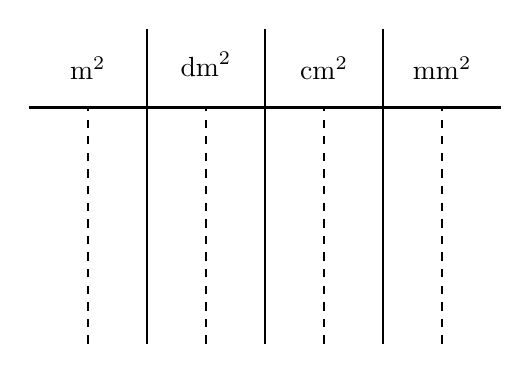
\begin{tikzpicture}[scale=1, every node/.style={scale=1}]
        \draw[color = black, smooth, thick, dashed] (-0.75,0) -- (-0.75,3);
        \draw[color = black, smooth, thick] (0,0) -- (0,4);
        \draw[color = black, smooth, thick, dashed] (0.75,0) -- (0.75,3);
        \draw[color = black, smooth, thick] (1.5,0) -- (1.5,4);
        \draw[color = black, smooth, thick, dashed] (2.25,0) -- (2.25,3);
        \draw[color = black, smooth, thick] (3,0) -- (3,4);
        \draw[color = black, smooth, thick, dashed] (3.75,0) -- (3.75,3);
        \draw[color = black, smooth, thick] (-1.5,3) -- (4.5,3);
        \node at (-0.75,3.5) {$\mathrm{m}^{2}$};
        \node at (0.75,3.55) {$\mathrm{dm}^{2}$};
        \node at (2.25,3.5) {$\mathrm{cm}^{2}$};
        \node at (3.75,3.5) {$\mathrm{mm}^{2}$};
        \end{tikzpicture}
    \end{center}
    Hetzelfde geldt voor volumematen, alleen moet je nu elke kolom in drie splitsen:
    \begin{center}
        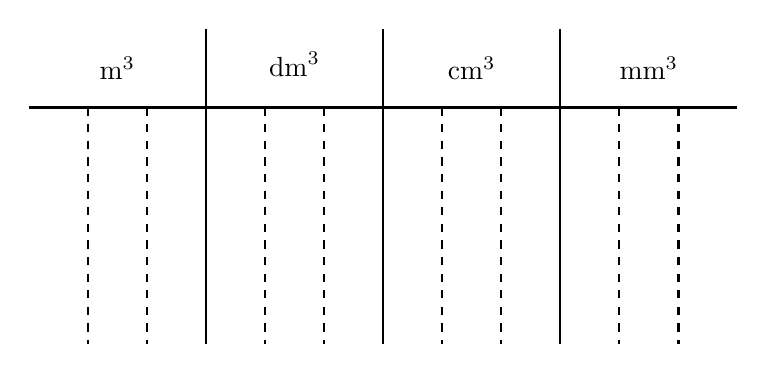
\begin{tikzpicture}[scale=1, every node/.style={scale=1}]
        \draw[color = black, smooth, thick] (0,0) -- (9,0);
        \draw[color = black, smooth, thick, dashed] (0.75,0) -- (0.75,-3);
        \draw[color = black, smooth, thick, dashed] (1.5,0) -- (1.5,-3);
        \draw[color = black, smooth, thick] (2.25,1) -- (2.25,-3);
        \draw[color = black, smooth, thick, dashed] (3,0) -- (3,-3);
        \draw[color = black, smooth, thick, dashed] (3.75,0) -- (3.75,-3);
        \draw[color = black, smooth, thick] (4.5,1) -- (4.5,-3);
        \draw[color = black, smooth, thick, dashed] (5.25,0) -- (5.25,-3);
        \draw[color = black, smooth, thick, dashed] (6,0) -- (6,-3);
        \draw[color = black, smooth, thick] (6.75,1) -- (6.75,-3);
        \draw[color = black, smooth, thick, dashed] (7.5,0) -- (7.5,-3);
        \draw[color = black, smooth, thick, dashed] (8.25,0) -- (8.25,-3);
        \node at (1.125,0.5) {$\mathrm{m}^{3}$};
        \node at (3.375,0.55) {$\mathrm{dm}^{3}$};
        \node at (5.625,0.5) {$\mathrm{cm}^{3}$};
        \node at (7.875,0.5) {$\mathrm{mm}^{3}$};
        \end{tikzpicture}
    \end{center}
    Eenheden omzetten met bovenstaande tabellen werkt en is zeker juist, maar wanneer je bijvoorbeeld van kubieke gigameter naar kubieke nanometer moet overgaan, kan deze methode best omslachtig zijn. Daarom is het ook hier \underline{sterk aangeraden} om eenheden om te zetten door gebruik te maken van machten van 10.
\end{remark}

Volumematen worden vaak uitgedrukt in $\mathrm{m}^{3}$, samen met een bijhorende prefix. Wanneer je echter met vloeistoffen werkt, zal je vaak in contact komen met een andere eenheid voor volume, namelijk de liter.

\begin{definition}\nl
    De \textbf{liter} (symbool: L of l) is een eenheid voor volume. \\
    Per definitie geldt er dat $1 \, \mathrm{L} = 1 \, \mathrm{dm}^{3}$. Merk op dat deze gelijkheid niet alleen voor water geldt, maar voor eender welke (vloei)stof!

    \begin{remark}
        Zowel een hoofdletter L als een kleine letter l wordt gebruikt voor liter, maar vaak gaat de voorkeur uit naar de hoofdletter L als symbool om mogelijke verwarring met het cijfer 1 te vermijden.
    \end{remark}
\end{definition}

\begin{example}[foldable=true,title={Voorbeeld: Omzetten van cL naar kubieke millimeter}]\nl
    Een fles wijn bevat typisch $75 \, \mathrm{cL}$ wijn. Hoeveel kubieke millimeter is dit?

    \begin{solution}\nl
        We weten dat $1 \, \mathrm{L} = 1 \, \mathrm{dm}^{3}$. Verder kunnen we in de tabel met prefixen aflezen dat deci gelijk aan $10^{-1}$ is, centi gelijk aan $10^{-2}$ is en milli $10^{-3}$ is. Bijgevolg vinden we dat:
        \begin{align*}
        1 \, \mathrm{L} & = 1 \, \mathrm{dm}^{3} & \\
        1 \, \mathrm{L} & = 1\, (\textcolor{red}{\mathrm{d}}\mathrm{m})^{3} & \\
        1 \, \mathrm{L} & = 1 \cdot (\textcolor{red}{10^{-1}} \, \mathrm{m})^{3} & \\
        1 \, \mathrm{L} & = 1 \cdot 10^{-3} \, \mathrm{m}^{3} & \\
        \textcolor{green}{10^{-2}} \, \mathrm{L} & = 10^{-2} \cdot 10^{-3} \, \mathrm{m}^{3} & (\text{\textit{Beide leden}} \cdot 10^{-2}) \\
        1 \, \textcolor{green}{\mathrm{c}}\mathrm{L} & = 10^{-5} \, \mathrm{m}^{3} & \\
        10^{-9} \, \mathrm{cL} & = 10^{-9} \cdot 10^{-5} \, \mathrm{m}^{3} & (\text{\textit{Beide leden}} \cdot 10^{-9}) \\
        10^{-9} \, \mathrm{cL} & = 10^{-5} \cdot (10^{-3})^{3} \, \mathrm{m}^{3} & \\
        10^{-9} \, \mathrm{cL} & = 10^{-5} \cdot (\textcolor{blue}{10^{-3}} \, \mathrm{m})^{3} & \\
        10^{-9} \, \mathrm{cL} & = 10^{-5} \, (\textcolor{blue}{\mathrm{m}}\mathrm{m})^{3} & \\
        10^{-9} \, \mathrm{cL} & = 10^{-5} \, \mathrm{mm}^{3} & \\
        75 \cdot 10^{-9} \, \mathrm{cL} & = 75 \cdot 10^{-5} \, \mathrm{mm}^{3} & (\text{\textit{Beide leden}} \cdot 75) \\
        75 \, \mathrm{cL} & = \frac{75 \cdot 10^{-5}}{10^{-9}} \, \mathrm{mm}^{3} & \\
        75 \, \mathrm{cL} & = 75 \cdot 10^{4} \, \mathrm{mm}^{3} & \\
        \end{align*}
    \end{solution}
\end{example}

\section{Omzetten van eenheden met breuken}
Tot hiertoe hebben we steeds voorbeelden besproken van lengtes en massa's, maar in fysica bestaan er heel wat grootheden die een breuk als eenheid hebben. Denk maar bijvoorbeeld aan snelheid of massadichtheid. Ook wanneer eenheden als breuk genoteerd staan, moet je de nodige omzettingen kunnen maken.

Het omzetten van eenheden die uit breuken bestaan, is heel gelijkaardig aan het letterrekenen in wiskunde: Beschouw eenheden als letters/symbolen en pas vervolgens de rekenregels toe die je gewoon bent vanuit de lessen wiskunde.

\begin{example}[foldable=true,title={Voorbeeld: km/h naar m/s}]\nl
    Een auto heeft een snelheid van $50{,}0 \, \mathrm{km/h}$. Hoeveel m/s is dit?

    \begin{solution}\nl
        We behandelen de $\mathrm{km/h}$ en de $\mathrm{m/s}$ als breuken zoals je in de lessen wiskunde zou doen. Zo vinden we dat:
        \begin{align*}
        50{,}0 \, \mathrm{km/h} & = \frac{50{,}0 \, \mathrm{km}}{\mathrm{h}} \\
        & = \frac{50{,}0 \cdot 10^{3} \, \mathrm{m}}{\mathrm{h}} \\
        & = \frac{50{,}0 \cdot 10^{3} \, \mathrm{m}}{60 \, \mathrm{min}} \\
        & = \frac{50{,}0 \cdot 10^{3} \, \mathrm{m}}{60 \cdot 60 \, \mathrm{s}} \\
        & = \frac{50{,}0 \cdot 10^{3}}{60 \cdot 60} \cdot \frac{\mathrm{m}}{\mathrm{s}} \\
        & \approx 13{,}9 \, \mathrm{m/s}.
        \end{align*}
        In deze uitwerking hebben we gebruikt dat $1 \, \mathrm{h} = 60$ minuten en dat $1 \text{ minuut} = 60$ seconden, wat bijgevolg betekent dat $1 \, \mathrm{h} = 60 \cdot 60$ seconden. In de volgende sectie zal het omzetten van uren, minuten en seconden uitgebreider besproken worden.
    \end{solution}
\end{example}

\begin{example}[foldable=true,title={Voorbeeld: Omzetten van Massadichtheid}]\nl
    Een voorwerp heeft een massadichtheid van $3{,}0 \, \mathrm{kg/m}^{3}$. Hoeveel g/cm$^{3}$ is dit?

    \begin{solution}\nl
        We gaan op dezelfde manier te werk zoals bij het vorige voorbeeld. We vinden bijgevolg dat:
        \begin{align*}
        3{,}0 \, \mathrm{kg/m}^{3} & = \frac{3{,}0 \, \mathrm{kg}}{\mathrm{m}^{3}} \\
        & = \frac{3{,}0 \cdot 10^{3} \, \mathrm{g}}{\mathrm{m}^{3}} \\
        & = \frac{3{,}0 \cdot 10^{3} \cdot 10^{-6} \, \mathrm{g}}{10^{-6}\, \mathrm{m}^{3}} & (\text{\textit{Teller en noemer}} \cdot 10^{-6}) \\
        & = \frac{3{,}0 \cdot 10^{-3} \, \mathrm{g}}{(10^{-2})^{3} \, \mathrm{m}^{3}} \\
        3{,}0 \, \mathrm{kg/m}^{3} & = \frac{3{,}0 \cdot 10^{-3} \, \mathrm{g}}{(10^{-2} \, \mathrm{m})^{3}} \\
        & = \frac{3{,}0 \cdot 10^{-3} \, \mathrm{g}}{(\mathrm{cm})^{3}} \\
        & = 3{,}0 \cdot 10^{-3} \, \mathrm{g/cm}^{3}.
        \end{align*}
    \end{solution}
\end{example}

\section{Omzetten van dagen, uren, minuten en seconden}
Het omzetten van eenheden voor tijd, zoals jaren, maanden, uren, minuten, seconden,... verloopt lichtelijk anders vergeleken met de omzettingen die we tot hiertoe gemaakt hebben. Het verschil hierbij is dat we niet met machten van 10 kunnen werken, maar bijvoorbeeld moeten nagaan hoeveel uren er in een dag zitten of hoeveel minuten er in een uur kunnen. Volgende voorbeelden illustreren dit.

\begin{example}[foldable=true,title={Voorbeeld: Aantal Seconden in een Dag}]\nl
    Hoeveel seconden duurt een dag?

    \begin{solution}\nl
        Eén dag bestaat uit $24\,\mathrm{h}$, één uur uit 60 minuten en één minuut uit 60 seconden. Bijgevolg is:
        \begin{align*}
        1 \text{ dag} & = 24 \, \mathrm{h} \\
        & = 24 \cdot \textcolor{red}{1 \, \mathrm{h}} \\
        & = 24 \cdot \textcolor{red}{60 \text{ minuten}} \\
        & = 24 \cdot 60 \cdot \textcolor{green}{1 \text{ minuut}} \\
        & = 24 \cdot 60 \cdot \textcolor{green}{60 \text{ seconden}}
        \end{align*}
        en vinden we dus dat $1 \text{ dag} = 86400 \text{ seconden}$.
    \end{solution}
\end{example}

\begin{example}[foldable=true,title={Voorbeeld: Uur naar uur, minuten en seconden omzetten}]\nl
    Je meet een tijd van $8{,}43$ uur. Hoeveel uren, minuten en seconden zijn dit?

    \begin{solution}\nl
        We weten met zekerheid dat we al minstens een tijd van 8 uur hebben. De vraag die we ons nu nog moeten stellen, is hoeveel minuten en seconden $0{,}43$ uur is.

        Omdat $1 \, \mathrm{h} = 60 \text{ minuten}$, zal 
        \begin{align*}
        0{,}43 \, \mathrm{h} & = 0{,}43 \cdot 60 \text{ minuten} \\
        & = 25{,}8 \text{ minuten}.
        \end{align*}
        We weten hierdoor dat we bovenop de 8 uur een extra 25 minuten gemeten hebben. Al wat ons nu nog rest, is om op een analoge manier te werk te gaan om zo te achterhalen hoeveel seconden $0{,}8$ minuten zijn.

        Bijgevolg, omdat $1 \text{ minuut} = 60 \text{ seconden}$, vinden we dat:
        \begin{align*}
        0{,}8 \text{ minuten} & = 0{,}8 \cdot 60 \text{ seconden} \\
        & = 48 \text{ seconden}
        \end{align*}
        We hebben hierdoor gevonden dat $8{,}43$ uur gelijk is aan 8 uur, 25 minuten en 48 seconden.
    \end{solution}
\end{example}

\begin{example}[foldable=true,title={Voorbeeld: Minuten en seconden naar uur omzetten}]\nl
    Je meet een tijd van $3{,}0$ minuten en 13 seconden. Hoeveel uur is dit?

    \begin{solution}\nl
        We gaan op dezelfde manier te werk zoals bij het vorige voorbeeld. We weten dat $1 \, \mathrm{h} = 60 \text{ minuten}$. Bijgevolg is:
        \begin{align*}
        1 \, \mathrm{h} & = 60 \text{ minuten} \\
        \frac{1}{60} \, \mathrm{h} & = 1 \text{ minuut} \\
        3 \text{ minuten} & = 3 \cdot \frac{1}{60} \, \mathrm{h} & (\text{\textit{Beide leden}} \cdot 3) \\
        3 \text{ minuten} & = 0{,}05 \, \mathrm{h}
        \end{align*}
        Op een gelijkaardige manier vinden we dan dat:
        \begin{align*}
        1 \, \mathrm{h} & = 60 \text{ minuten} \\
        1 \, \mathrm{h} & = 60 \cdot 60 \text{ seconden} \\
        1 \text{ seconde} & = \frac{1}{3600} \, \mathrm{h} \\
        13 \text{ seconden} & = 13 \cdot \frac{1}{3600} \, \mathrm{h} & (\text{\textit{Beide leden}} \cdot 13) \\
        13 \text{ seconden} & \approx 0{,}0036 \, \mathrm{h}
        \end{align*}
        Bijgevolg is $3{,}0$ minuten en 13 seconden gelijk aan $0{,}05 \, \mathrm{h} + 0{,}0036 \, \mathrm{h} = 0{,}0536 \, \mathrm{h}$.
    \end{solution}
\end{example}

\end{document}